\documentclass[11pt]{article}

\usepackage[margin=1in]{geometry}
\usepackage[T1]{fontenc}
\usepackage{lmodern}
\usepackage{amsmath,amssymb,amsthm,bm}
\usepackage{booktabs}
\usepackage{graphicx}
\usepackage{adjustbox}
\usepackage{algorithm}
\usepackage{algpseudocode}
\usepackage{xcolor}
\usepackage[hidelinks]{hyperref}
\usepackage[style=authoryear,maxcitenames=2,maxbibnames=10,uniquename=false,uniquelist=false,backend=biber]{biblatex}
\addbibresource{references.bib}
\appto{\bibsetup}{\sloppy}
\graphicspath{{../results/figures/}}

\setlength{\parskip}{0.4em}
\setlength{\parindent}{0pt}

\newtheorem{proposition}{Proposition}
\newtheorem{corollary}{Corollary}
\theoremstyle{remark}
\newtheorem{remark}{Remark}

\newcommand{\E}{\mathbb{E}}

\title{Cutting Planes Are Costates: Neural Stochastic Dual Dynamic\\ Programming for the Analytic Climate Economy}
\author{Herman Vestvik Thieme}
\date{\today \\[0.5em] \textit{Draft}}

\begin{document}
\maketitle

\begin{abstract}
Stochastic dual dynamic programming (SDDP) approximates the value function of a multistage problem by cutting planes, and neural SDDP learns those cutting planes across problem instances. I apply both to the Analytic Climate Economy (ACE), an integrated assessment model with DICE functional forms and a closed-form solution, so that every result can be checked exactly. With business-as-usual emissions on an exogenous path, each period of ACE is a small convex program, and the gradient of its value, obtained from the multipliers on the cuts, is the costate recursion of the model's equilibrium conditions: the slopes of the cuts are ACE's costates, and the social cost of carbon (SCC) follows from them. Because ACE's value function is affine, SDDP is exact after two iterations; it reproduces the closed-form SCC to within 0.002\% across a wide range of time preferences, damages and carbon-cycle parameters, in under three seconds per parameter draw. A cut network trained on 128 SDDP solutions predicts the cuts for new parameter values; one forward pass with these cuts, without any SDDP iterations, gives the SCC with a median error of 0.2\% (at most 2.5\%), 8 to 19 times more accurate than a pseudo-state deep equilibrium net on the same test draws. Warm-starting SDDP with the predicted cuts makes its first policy nearly optimal but does not reduce the number of iterations, because SDDP from scratch already needs only one backward pass. I discuss what these results imply for climate-economy models without closed forms, where curved value functions would let neural SDDP pay off, and where non-convexities such as tipping points would break SDDP's guarantees.

\end{abstract}

\section{Introduction}
\label{sec:introduction}

Integrated assessment models (IAMs) link a model of the economy to a model of the climate and ask what a tonne of carbon dioxide costs society. Their answer, the social cost of carbon (SCC), is a shadow price: the marginal value of carbon in the atmosphere, relative to the marginal value of consumption. Computing it requires solving a dynamic optimisation problem over centuries, and the moment such a problem has more than a handful of state variables, or uncertainty, or tipping points, conventional grid-based dynamic programming runs into the curse of dimensionality. A growing literature therefore turns to methods from machine learning: deep equilibrium nets, which train a network to satisfy a model's equilibrium conditions \parencite{Azinovic2022DEQN,Maliar2021,Folini2024ClimateInCE}, their extension to uncertain parameters \parencite{friedl2023_deepUQ}, and reinforcement learning.

Operations research has a different and much older answer to the same problem. Stochastic dual dynamic programming (SDDP) \parencite{PereiraPinto1991} solves multistage stochastic programs, originally for hydrothermal power systems, by approximating each stage's value function from above with cutting planes \parencite{Kelley1960,Benders1962}. It alternates forward passes, which simulate the policy implied by the current cuts, with backward passes, which add a cut at each visited state using the value and the gradient of the stage problem. It needs convexity, but where convexity holds it comes with bounds on the optimum and convergence guarantees \parencite{Shapiro2011,Girardeau2015}. Neural SDDP \parencite{Dai2022NeuralSDDP} adds a network that maps a problem instance to its cuts, trained on earlier solutions, so that new instances can be solved faster or without iterations at all.

This paper applies both methods to the Analytic Climate Economy (ACE) of \textcite{TraegerChristian2023ACE}, in the DICE calibrations used by \textcite{traeger2021analytic_discussion}. ACE keeps the DICE production function, carbon cycle and temperature dynamics, but transforms capital and temperature so that the value function is affine and the model has a closed-form solution. That makes it a demanding benchmark: every number a method produces can be compared with the exact one.

The contributions are the following.

\begin{enumerate}
    \item \textbf{ACE as a sequence of convex programs.} With business-as-usual emissions on an exogenous path, which is the assumption behind ACE's closed form, each period's problem is convex as long as the cuts value capital positively (Proposition~\ref{prop:convex}). The gradient of the stage value, obtained from the multipliers on the cuts by the envelope theorem, is exactly the costate recursion of the model's equilibrium conditions (Proposition~\ref{prop:gradient}). The slopes of the cuts are therefore ACE's costates, and the SCC follows from the slopes of the next period's cut. This is a third route to the same shadow prices, next to the residuals of the equilibrium conditions used by deep equilibrium nets and the gradient of a learned value function used by actor-critic methods. Proposition~\ref{prop:convex}, the concavity of every value function on which the validity of the cuts rests, and the closed-form facts behind Proposition~\ref{prop:fixed} and Remark~\ref{rem:truncation} are verified formally in Lean (Appendix~\ref{app:lean}).
    \item \textbf{SDDP is exact in two iterations.} Because the value function is affine, a cut computed at any state is exact, the closed-form cut is a fixed point of the backward pass (Proposition~\ref{prop:fixed}), and SDDP from scratch converges after one backward pass (Corollary~\ref{cor:two}). Across 256 test draws of the time preference, the damage coefficient and the speed of atmosphere--ocean carbon exchange, it reproduces the closed-form SCC to within 0.002\%, in under three seconds per draw.
    \item \textbf{Neural SDDP predicts the cuts across parameter values.} A cut network trained on the SDDP solutions of 128 parameter draws gives, with a single forward pass and no SDDP iterations, a median SCC error of 0.24\% (DICE 2016) and 0.21\% (DICE 2023), at most 2.5\%, and a welfare loss below 0.0006\% on every test draw. On the same draws, this is 8 to 19 times more accurate than a pseudo-state deep equilibrium net trained over the same parameter box.
    \item \textbf{Warm starts do not help in ACE, and I explain why.} The predicted cuts make the first forward pass nearly optimal, within $10^{-9}$ of the optimum against 12\% below it from scratch. But certifying convergence requires a backward pass either way, and from scratch SDDP needs only one. The speed-ups of neural SDDP require value functions that need many cuts.
    \item \textbf{Uncertainty and the horizon.} With i.i.d.\ productivity shocks, SDDP proper (averaging cuts over shocks, sampling them forward) recovers the same costates and policy, as ACE predicts. The horizon after which the value is set to zero has to be long at low discount rates, because carbon's shadow price converges only at the rate $\beta$ (Remark~\ref{rem:truncation}).
\end{enumerate}

The paper is organised as follows. Section~\ref{sec:related} reviews related work. Section~\ref{sec:model} presents the model and its closed form. Section~\ref{sec:method} formulates the stage problems, derives the cuts and describes SDDP and neural SDDP. Section~\ref{sec:setup} describes the experiments, Section~\ref{sec:results} the results, and Section~\ref{sec:discussion} discusses what they imply for models without closed forms.

\section{Related Work}
\label{sec:related}

\paragraph{SDDP.} SDDP was introduced by \textcite{PereiraPinto1991} for the planning of hydrothermal power systems, building on the cutting-plane method of \textcite{Kelley1960} and the decomposition of \textcite{Benders1962}. \textcite{Shapiro2011} analyses its statistical properties and stopping rules, and \textcite{Girardeau2015} prove convergence for multistage stochastic convex programs, the setting of this paper; \textcite{DowsonKapelevich2021} provide a widely used implementation. SDDP relies on convexity of the value functions in the state and on stagewise-independent uncertainty; both hold in ACE with exogenous business-as-usual emissions and i.i.d.\ shocks.

\paragraph{Learning value functions for multistage problems.} \textcite{Dai2022NeuralSDDP} introduce neural SDDP ($\nu$-SDDP), in which a network maps a problem instance to a piecewise-linear value function in a learned low-dimensional projection of the state, and use it to warm-start or replace SDDP on new instances. Related approaches learn the gradients of the value function \parencite{Lee2023VFGL}, represent it with input-convex neural networks \parencite{Bae2023DVFN}, or generate cuts sequentially with a transformer \parencite{Kim2023TranSDDP}. These papers evaluate their methods on inventory, production and energy planning problems against SDDP solutions; here the benchmark is a closed form.

\paragraph{Solving IAMs.} Analytic IAMs include \textcite{Golosov2014} and ACE \parencite{TraegerChristian2023ACE}. Numerical approaches include dynamic programming with risk \parencite{CaiLontzek2019} and tipping points \parencite{LemoineTraeger2014}, and deep learning: deep equilibrium nets \parencite{Azinovic2022DEQN}, applied to climate economics by \textcite{Folini2024ClimateInCE}, and deep uncertainty quantification, which treats uncertain parameters as pseudo-states \parencite{friedl2023_deepUQ}. The companion revision of the thesis behind this repository \parencite{Thieme2025Revised} corrects the equilibrium conditions of a deep equilibrium net for ACE; its pseudo-state extension is the comparison in Section~\ref{sec:results}. To my knowledge, SDDP and neural SDDP have not been applied to an IAM with a closed-form benchmark.

\section{The Analytic Climate Economy}
\label{sec:model}

I use ACE \parencite{TraegerChristian2023ACE} with the DICE production function, carbon cycle and two-layer temperature model, in the calibrations of DICE 2016 \parencite{NordhausWilliam2018PaUa} and DICE 2023 \parencite{NordhausWilliam2023}, following \textcite{traeger2021analytic_discussion}. Time is discrete, with periods of $\Delta = 5$ years.

\paragraph{States, decisions and reward.} The state is $\bm{s}_t = (k_t, \bm{M}_t, \bm{\tau}_t) \in \mathbb{R}^6$, where $k_t = \log K_t$ is log capital, $\bm{M}_t \in \mathbb{R}^3$ are the carbon stocks in the atmosphere, upper ocean and deep ocean (GtC), and $\bm{\tau}_t \in \mathbb{R}^2$ are transformed atmospheric and ocean temperatures, $\tau_{i,t} = \exp(\xi_1 T_{i,t})$. In each period the planner chooses the consumption rate $x_t \in (0, 1)$ and the abatement rate $\mu_t \in [0, 1]$. Log output net of abatement costs and damages is
\begin{equation}
    g_t(\bm{s}_t, \mu_t) = \log A_t + (1-\kappa)\log N_t + \kappa k_t + \log\left(1 - \theta_{1,t}\mu_t^{\theta_2}\right) - \xi_0 \tau_{1,t} + \xi_0,
    \label{eq:g}
\end{equation}
with exogenous productivity $A_t$, labour $N_t$ and abatement-cost coefficients $\theta_{1,t}$ from DICE, and $\theta_2 = 2.6$. The reward is log consumption, $u_t = \log x_t + g_t(\bm{s}_t, \mu_t)$, and the planner maximises $\sum_t \beta^t u_t$ with $\beta = (1+\rho)^{-\Delta}$.

\paragraph{Laws of motion.} Capital, carbon and temperatures evolve as
\begin{align}
    k_{t+1} &= g_t(\bm{s}_t, \mu_t) + \log(1 - x_t) + c_k, \label{eq:k} \\
    \bm{M}_{t+1} &= \bm{\Phi}\bm{M}_t + \bm{e}_1 \zeta \left[(1-\mu_t)E^{\text{BAU}}_t + E^{\text{land}}_t\right], \label{eq:M} \\
    \bm{\tau}_{t+1} &= \bm{\sigma}\bm{\tau}_t + \bm{e}_1 \sigma^{\text{forc}} \frac{M_{1,t}}{M_{\text{pre}}}, \label{eq:tau}
\end{align}
where $c_k = \log[(1 + g_k\Delta)/(\delta_k + g_k)]$, emissions are measured in GtCO$_2$ per year and $\zeta = \Delta/3.664$ converts them into GtC per period. The carbon transition matrix $\bm{\Phi}$ is column-stochastic: it moves carbon between reservoirs and conserves it.

\paragraph{Business-as-usual emissions.} In DICE, business-as-usual emissions are proportional to gross output, $E^{\text{BAU}}_t = \sigma_t Y^{\text{gross}}_t$, and so depend on capital. ACE's closed form requires the planner to take them as given. As in the actor-critic paper of this series, I fix $E^{\text{BAU}}_t$ to an exogenous reference path: carbon intensity times gross output along the optimal path at baseline parameters. The problem solved by SDDP and the problem with the closed-form solution are then the same.

\paragraph{Uncertain parameters.} Three parameters vary across instances, over the box used for deep uncertainty quantification in this series: the pure rate of time preference $\rho \in [0.5\%, 3.5\%]$ per year, the damage coefficient $\xi_0 \in [0.011, 0.044]$ (half to twice its baseline), and a multiplier $\omega \in [0.75, 1.25]$ on the exchange of carbon between the atmosphere and the upper ocean, which scales the two corresponding entries of $\bm{\Phi}$ and keeps it column-stochastic. I write $\bm{p} = (\rho, \xi_0, \omega)$ for an instance.

\paragraph{Closed form.} The value function is affine, $V_t(\bm{s}) = \alpha_t + \bm{b}^\top \bm{s}$, with slopes that are constant over time:
\begin{align}
    b_k &= \frac{\kappa}{1-\beta\kappa}, \label{eq:bk} \\
    \bm{b}_\tau &= -\xi_0(1+\beta b_k)\left(\bm{I} - \beta\bm{\sigma}^\top\right)^{-1}\bm{e}_1, \label{eq:btau} \\
    \bm{b}_M &= \beta\frac{\sigma^{\text{forc}}}{M_{\text{pre}}}\, b_{\tau_1}\left(\bm{I} - \beta\bm{\Phi}^\top\right)^{-1}\bm{e}_1 . \label{eq:bM}
\end{align}
In the notation of the deep equilibrium nets in this series, the costates are $\bm{\lambda} = \beta\bm{b}$. The optimal consumption rate is $x^* = 1/(1 + \beta b_k) = 1 - \beta\kappa$, and the optimal abatement rate equates the marginal product of emissions to the carbon price,
\begin{equation}
    \frac{\theta_{1,t}\theta_2 \mu_t^{\theta_2 - 1}}{E^{\text{BAU}}_t\left(1 - \theta_{1,t}\mu_t^{\theta_2}\right)} = p^C \equiv -\frac{\zeta \beta b_{M_1}}{1+\beta b_k},
    \label{eq:mu}
\end{equation}
with $\mu^*_t = 1$ where the solution would exceed one. The SCC in USD per tCO$_2$ is
\begin{equation}
    SCC_t = 1000\, Y^{\text{net}}_t\, p^C = -1000\, Y^{\text{net}}_t\, \frac{\zeta \beta b_{M_1}}{1 + \beta b_k},
    \label{eq:scc}
\end{equation}
where $Y^{\text{net}}_t = \exp(g_t)$ is net output in trillion USD.

\section{Method}
\label{sec:method}

\subsection{Stage problems}

Let $\mathcal{C}_{t+1}$ be a set of cuts $(\alpha_j, \bm{b}_j)$ with $V_{t+1}(\bm{s}) \le \alpha_j + \bm{b}_j^\top\bm{s}$. Writing $\bm{f}_t(\bm{s}, x, \mu)$ for the laws of motion \eqref{eq:k}--\eqref{eq:tau}, the stage problem at state $\bm{s}$ is
\begin{equation}
\begin{aligned}
    \hat V_t(\bm{s}) = \max_{x, \mu, \theta}\quad & \log x + g_t(\bm{s}, \mu) + \beta\theta \\
    \text{s.t.}\quad & \theta \le \alpha_j + \bm{b}_j^\top \bm{f}_t(\bm{s}, x, \mu), \qquad j \in \mathcal{C}_{t+1}, \\
    & \underline{x} \le x \le \overline{x}, \quad 0 \le \mu \le 1 .
\end{aligned}
\tag{P$_t$}
\label{eq:stage}
\end{equation}

\begin{proposition}[Convexity]
\label{prop:convex}
If every cut has $b_{j,k} \ge 0$, problem \eqref{eq:stage} is a convex program.
\end{proposition}

\begin{proof}
Since $\theta_2 > 1$, $\mu^{\theta_2}$ is convex on $[0,1]$, so $\log(1 - \theta_{1,t}\mu^{\theta_2})$ is concave, and with $\log x$ and $\log(1-x)$ the objective and next capital \eqref{eq:k} are concave in $(x, \mu)$. Next carbon \eqref{eq:M} is affine in $\mu$, and next temperatures \eqref{eq:tau} do not depend on the decisions. The right-hand side of each cut constraint is therefore concave when $b_{j,k} \ge 0$, and the feasible set $\{\theta \le \text{concave}\}$ is convex.
\end{proof}

The condition $b_{j,k} \ge 0$ says that capital is valuable. It holds for every cut SDDP computes, and I enforce it for predicted cuts: by backward induction from $V_T = 0$, every value function of ACE is concave in the state and nondecreasing in capital, so every cut computed from its value and gradient is a valid upper bound with $b_k \ge 0$. Proposition~\ref{prop:convex} and this induction are proved formally in Lean (Appendix~\ref{app:lean}). I implement \eqref{eq:stage} once in CVXPY \parencite{DiamondBoyd2016} in disciplined parametrised form \parencite{Agrawal2019DPP}, introducing auxiliary variables $w \le \log(1-\theta_{1,t}\mu^{\theta_2})$ and $z \le w + \log(1-x)$ so that the cut slopes on capital multiply a variable rather than an expression with parameters. The problem is then re-solved with new parameters for every stage, state and cut set, with the interior-point solver Clarabel \parencite{GoulartChen2024Clarabel}.

\subsection{Cuts from duals}

\begin{proposition}[Cut gradient]
\label{prop:gradient}
Let $\pi_j \ge 0$ be the multipliers of the cut constraints at a solution of \eqref{eq:stage}; they satisfy $\sum_j \pi_j = \beta$. Define $w_k = \sum_j \pi_j b_{j,k}$, $\bm{w}_M = \sum_j \pi_j \bm{b}_{j,M}$ and $\bm{w}_\tau = \sum_j \pi_j \bm{b}_{j,\tau}$. Then
\begin{align}
    \frac{\partial \hat V_t}{\partial k} &= \kappa\,(1 + w_k), \\
    \frac{\partial \hat V_t}{\partial \bm{M}} &= \bm{\Phi}^\top \bm{w}_M + \frac{\sigma^{\text{forc}}}{M_{\text{pre}}}\, w_{\tau_1}\, \bm{e}_1, \\
    \frac{\partial \hat V_t}{\partial \bm{\tau}} &= \bm{\sigma}^\top \bm{w}_\tau - \xi_0\,(1 + w_k)\,\bm{e}_1 .
\end{align}
\end{proposition}

\begin{proof}
Stationarity of the Lagrangian in $\theta$ gives $\sum_j \pi_j = \beta$. The state enters \eqref{eq:stage} only through $g_t$ and $\bm{f}_t$, so by the envelope theorem $\nabla_{\bm{s}} \hat V_t = \nabla_{\bm{s}} g_t + \sum_j \pi_j\, \bm{J}_t^\top \bm{b}_j$, where $\bm{J}_t$ is the Jacobian of $\bm{f}_t$ with respect to the state: $\partial k_{t+1}/\partial k_t = \kappa$, $\partial k_{t+1}/\partial \tau_{1,t} = -\xi_0$, $\partial \bm{M}_{t+1}/\partial \bm{M}_t = \bm{\Phi}$, $\partial \tau_{1,t+1}/\partial M_{1,t} = \sigma^{\text{forc}}/M_{\text{pre}}$ and $\partial \bm{\tau}_{t+1}/\partial\bm{\tau}_t = \bm{\sigma}$. Collecting terms gives the result.
\end{proof}

With $\bm{\lambda}_t = \sum_j \pi_j \bm{b}_j = (w_k, \bm{w}_M, \bm{w}_\tau)$, these are the costate equations of ACE: $\lambda_{k,t-1} = \beta\kappa(1 + \lambda_{k,t})$ and its counterparts for carbon and temperature, which deep equilibrium nets enforce as residuals. A backward pass of SDDP evaluates them from the duals of convex programs. The new cut for $V_t$ at the visited state $\bm{s}$ is $(\hat V_t(\bm{s}) - \nabla\hat V_t^\top \bm{s},\ \nabla \hat V_t)$, and the SCC in period $t$ follows from \eqref{eq:scc} with the multiplier-weighted slopes $\bm{\lambda}_t / \beta$ of the next period's cuts.

\begin{proposition}[The closed form is a fixed point]
\label{prop:fixed}
If $\mathcal{C}_{t+1}$ consists of the single cut $(\alpha, \bm{b})$ with $\bm{b}$ from \eqref{eq:bk}--\eqref{eq:bM} and any $\alpha$, then \eqref{eq:stage} is solved by $x = 1 - \beta\kappa$ and the abatement rate $\mu^*_t$ of \eqref{eq:mu}, at every state, and its gradient is $\bm{b}$.
\end{proposition}

\begin{proof}
With one cut, $\pi = \beta$ and $\bm{\lambda}_t = \beta\bm{b}$. The first-order condition for $x$ is $1/x = \beta b_k/(1-x)$, so $x = 1/(1+\beta b_k) = 1 - \beta\kappa$; the condition for $\mu$ is \eqref{eq:mu}. Neither depends on the state. By Proposition~\ref{prop:gradient}, $\partial \hat V_t/\partial k = \kappa(1 + \beta b_k) = b_k$ by \eqref{eq:bk}; $\partial \hat V_t/\partial \bm{\tau} = \beta\bm{\sigma}^\top\bm{b}_\tau - \xi_0(1+\beta b_k)\bm{e}_1 = \bm{b}_\tau$ by \eqref{eq:btau}; and $\partial \hat V_t/\partial \bm{M} = \beta\bm{\Phi}^\top\bm{b}_M + \beta(\sigma^{\text{forc}}/M_{\text{pre}}) b_{\tau_1}\bm{e}_1 = \bm{b}_M$ by \eqref{eq:bM}.
\end{proof}

\begin{corollary}[Two iterations]
\label{cor:two}
In the deterministic problem truncated after $T$ stages with $V_T = 0$, and with exact stage solutions, SDDP started from any valid upper bound converges after two forward passes and one backward pass.
\end{corollary}

\begin{proof}
By the argument of Proposition~\ref{prop:fixed}, if $V_{t+1}$ is affine, the optimal decisions at stage $t$ do not depend on the state, and since the reward and the laws of motion are affine in the state for given decisions, $V_t$ is affine too. Starting from $V_T = 0$, every $V_t$ is affine, so the first backward pass, which proceeds from the last stage to the first, computes at each stage a cut that equals $V_t$ everywhere, whatever state it was computed at. The second forward pass then follows the optimal policy, and the cut at stage 0 equals the value of that policy.
\end{proof}

\begin{remark}[Truncation]
\label{rem:truncation}
The finite-horizon slopes follow the linear recursion of Proposition~\ref{prop:gradient} backwards from zero. The slope on capital converges at the rate $\beta\kappa$ per period and the slopes on temperature at a rate below $\beta$, but the slopes on carbon converge only at the rate $\beta$: $\bm{\Phi}$ is column-stochastic, so $\bm{\Phi}^\top$ has the eigenvalue one, the mode of carbon that is never removed from the system. The error in the SCC in period $t$ therefore decays like $\beta^{T-t}$. At $\rho = 0.5\%$ a year, $\beta = 0.975$ per period and $\beta^{150 - 58} \approx 0.10$, so a horizon of 150 periods is too short for an evaluation window of 58 periods; I use $T = 450$.
\end{remark}

\subsection{SDDP}

Algorithm~\ref{alg:sddp} summarises the method. Each stage starts with a provisional cut $V_{t} \le \bar V$; this cut, and any warm-start cuts, are replaced by the first cut a backward pass computes, so that only computed cuts determine the upper bound and later decisions. At most 16 cuts are kept per stage. The forward pass gives a lower bound $\underline{V}$, the value of a feasible policy; the stage-0 cuts evaluated at $\bm{s}_0$ give an upper bound $\bar V_0$; the algorithm stops when $(\bar V_0 - \underline{V})/|\underline{V}| < 10^{-7}$.

\begin{algorithm}[t]
\caption{SDDP for ACE}
\label{alg:sddp}
\begin{algorithmic}[1]
\State $\mathcal{C}_t \gets \{(\bar V, \bm{0})\}$ (provisional) for $t < T$; $\mathcal{C}_T \gets \{(0, \bm{0})\}$; optionally replace $\mathcal{C}_t$ by predicted cuts for $1 \le t < T$
\For{$i = 1, 2, \dots$}
    \State \textbf{Forward:} $\bm{s}_0$ given; for $t = 0, \dots, T-1$: solve (P$_t$) at $\bm{s}_t$ with $\mathcal{C}_{t+1}$, $\bm{s}_{t+1} \gets \bm{f}_t(\bm{s}_t, x_t, \mu_t)$
    \State $\underline{V} \gets \sum_t \beta^t u_t$; \quad $\bar V_0 \gets \min_{j \in \mathcal{C}_0} \alpha_j + \bm{b}_j^\top \bm{s}_0$
    \If{$(\bar V_0 - \underline{V}) / |\underline{V}| < \epsilon$} \textbf{stop} \EndIf
    \State \textbf{Backward:} for $t = T-1, \dots, 0$: solve (P$_t$) at $\bm{s}_t$ with $\mathcal{C}_{t+1}$; add the cut $(\hat V_t - \nabla\hat V_t^\top\bm{s}_t, \nabla\hat V_t)$ to $\mathcal{C}_t$, replacing provisional cuts
\EndFor
\end{algorithmic}
\end{algorithm}

\paragraph{Shocks.} To test the stochastic machinery, log productivity receives an i.i.d.\ shock $\varepsilon_t \sim \mathcal{N}(0, 0.03^2)$, observed before the decisions of period $t$. The backward pass then averages the values and gradients of \eqref{eq:stage} over five Gauss--Hermite nodes, the exact expectation for a polynomial of degree up to nine in the shock, and the forward pass samples the shocks. The shock enters $g_t$ additively, so it shifts the value function but not its slopes: the optimal policy is the same as without it.

\subsection{Neural SDDP}

The cut network $h_\omega(\bm{p}, t)$ maps an instance and a stage to a cut $(\hat\alpha_t, \hat{\bm{b}}_t)$. The slopes have fixed signs (capital is valuable, carbon and temperature are harmful) and span several orders of magnitude, from about 0.4 for capital to $10^{-8}$ for deep-ocean carbon, so the network predicts $\log|\bm{b}|$ and the intercept, each standardised over the training set. The error is then relative, the same for a low and a high SCC. The inputs are the parameters, scaled to $[-1, 1]$, and the stage. Unlike \textcite{Dai2022NeuralSDDP}, who predict several cuts in a learned low-dimensional space, I predict one cut per stage in the original state: ACE's value function is affine, and its state has only six dimensions.

The network is trained by supervised learning on the final cuts of SDDP solutions for training draws of $\bm{p}$, with a mean squared error. For a new instance it is used in two ways:
\begin{itemize}
    \item \textbf{No iterations:} one forward pass of Algorithm~\ref{alg:sddp} with the predicted cuts gives a policy, the SCC along the path and its value;
    \item \textbf{Warm start:} the predicted cuts replace the provisional cuts, and SDDP runs to convergence.
\end{itemize}

\section{Experimental Setup}
\label{sec:setup}

\paragraph{Instances.} For each calibration, DICE 2016 and DICE 2023, the training set consists of 128 instances and the test set of 256, drawn as scrambled Sobol sequences over the parameter box of Section~\ref{sec:model} with different seeds. The test draws are the same points as those used to evaluate the pseudo-state deep equilibrium net in this series, so the two methods are compared on identical instances.

\paragraph{SDDP.} The horizon is $T = 450$ periods; the evaluation window is the first 58 periods, up to about 2300. The consumption rate is bounded to $[0.2, 0.98]$, which never binds at the optimum, the provisional bound is $\bar V = 1000$, and the tolerance is $\epsilon = 10^{-7}$. A stage problem takes one to two milliseconds including Python overhead. Instances are solved in parallel in four processes on four CPU cores; the reported times per instance are the times within one process.

\paragraph{Cut network.} The network has three hidden layers of 128 units with swish activations and is trained with Adam \parencite{kingma2017adam} for 2{,}000 epochs, with batches of 1{,}024 and a learning rate decaying from $10^{-3}$ to $10^{-5}$ on a cosine schedule. Its training set has 57{,}600 rows: 450 stages for each of the 128 training instances. One seed is used per calibration.

\paragraph{Pseudo-state deep equilibrium net.} The comparison is the deep equilibrium net of the companion module on deep uncertainty quantification: a network with two hidden layers of 512 units that takes the state and the three parameters as inputs and is trained for 6{,}000 iterations on the corrected equilibrium conditions of ACE over the same parameter box. Its benchmark lets business-as-usual emissions move with capital in the laws of motion, while the planner takes them as given; the two benchmarks therefore differ slightly, but relative errors against each method's own closed form are comparable.

\paragraph{Metrics.} For every test instance I report, over the evaluation window, the mean relative error of the SCC along the path, the relative error of the SCC in the first period, the mean and maximum absolute errors of the abatement rate, the maximum absolute error of the consumption rate, and the consumption-equivalent welfare loss over the whole horizon, $\exp[(V^* - V)(1-\beta)] - 1$. Medians and maxima are taken over the 256 test instances.

\section{Results}
\label{sec:results}

Table~\ref{tab:accuracy} summarises the accuracy of each method on the 256 test instances, and Table~\ref{tab:cost} its cost.

\begin{table}[t]
\centering
\caption{Accuracy on 256 test instances: median over instances, with the maximum in parentheses. Errors are against the closed form over the periods up to about 2300.}
\label{tab:accuracy}
\begin{adjustbox}{max width=\textwidth}
\begin{tabular}{lcccc}
\toprule
 & SDDP & Neural SDDP, & Neural SDDP, & Pseudo-state \\
 & & no iterations & warm-started & DEQN \\
\midrule
\multicolumn{5}{l}{\textit{DICE 2016}} \\
SCC, mean relative error (\%) & 0.0007 (0.002) & 0.24 (2.1) & 0.0007 (0.002) & 1.8 (19) \\
SCC in the first period, relative error (\%) & 0.00001 (0.0008) & 0.37 (3.3) & 0.00001 (0.0008) & 2.0 (21) \\
Mean $|\mu - \mu^*|$ & 0.00001 (0.00003) & 0.0003 (0.003) & 0.00001 (0.00003) & 0.003 (0.028) \\
Max $|x - x^*|$ & 0.00002 (0.00005) & 0.00003 (0.00007) & 0.00002 (0.00005) & 0.006 (0.051) \\
Welfare loss (\%) & $<10^{-7}$ & $<0.0002$ & $<10^{-7}$ & -- \\
\midrule
\multicolumn{5}{l}{\textit{DICE 2023}} \\
SCC, mean relative error (\%) & 0.0007 (0.002) & 0.21 (2.5) & 0.0007 (0.002) & 4.0 (35) \\
SCC in the first period, relative error (\%) & 0.00001 (0.0008) & 0.26 (4.2) & 0.00001 (0.0008) & 3.6 (33) \\
Mean $|\mu - \mu^*|$ & 0.00001 (0.00002) & 0.0003 (0.004) & 0.00001 (0.00002) & 0.011 (0.059) \\
Max $|x - x^*|$ & 0.00002 (0.00003) & 0.00003 (0.0001) & 0.00002 (0.00004) & 0.010 (0.047) \\
Welfare loss (\%) & $<10^{-7}$ & $<0.0006$ & $<10^{-7}$ & -- \\
\bottomrule
\end{tabular}
\end{adjustbox}
\end{table}

\begin{table}[t]
\centering
\caption{Cost per test instance (median, one process) and training cost. Times for the two calibrations differ by less than 10\%; the table shows DICE 2016.}
\label{tab:cost}
\begin{tabular}{lccc}
\toprule
 & Iterations & Stage problems & Seconds \\
\midrule
SDDP from scratch & 2 & 1{,}350 & 2.5 \\
Neural SDDP, no iterations & -- & 450 & 0.9 \\
Neural SDDP, warm-started & 2 & 1{,}350 & 2.6 \\
\midrule
\multicolumn{4}{l}{\textit{Training (wall time on four cores)}} \\
SDDP solutions of 128 training instances & & & 90 \\
Cut network & & & 672 \\
Pseudo-state DEQN, for comparison & & & 3{,}170 \\
\bottomrule
\end{tabular}
\end{table}

\subsection{SDDP reproduces the closed form}

SDDP converges after two iterations on every instance, as Corollary~\ref{cor:two} predicts, with 1{,}350 stage problems: two forward passes and one backward pass over 450 stages. Its SCC matches the closed form to within 0.002\% on every test instance, its abatement rate to within $3 \times 10^{-4}$ and its consumption rate to within $5 \times 10^{-5}$ in every period; these residual errors are the solver's tolerance. The cut slopes agree with \eqref{eq:bk}--\eqref{eq:bM}: over the evaluation window, the largest relative deviation of any slope is $10^{-15}$ at baseline parameters and $8 \times 10^{-4}$ at the lowest discount rate and highest damages, where the truncation of Remark~\ref{rem:truncation} remains. The baseline SCC in 2050 is \$36.98 per tCO$_2$ for DICE 2016 and \$41.99 for DICE 2023, equal to the closed form to the cent.

Table~\ref{tab:truncation} shows why the horizon has to be long. With the lowest discount rate and the highest damages, a horizon of 150 periods leaves a mean SCC error of 4.2\% over the evaluation window, and 100 periods an error of 15\%; 450 periods bring it to 0.002\%. At the baseline and at high discount rates, 150 periods already suffice. The errors decay roughly like $\beta^{T-58}$, as Remark~\ref{rem:truncation} predicts.

\begin{table}[t]
\centering
\caption{Mean relative SCC error over the evaluation window (\%) for different horizons, DICE 2016.}
\label{tab:truncation}
\begin{tabular}{lccccc}
\toprule
Horizon $T$ (periods) & 100 & 150 & 250 & 350 & 450 \\
\midrule
$\rho = 0.5\%$, $\xi_0 \times 2$, $\omega = 0.75$ & 15.0 & 4.2 & 0.32 & 0.024 & 0.002 \\
Baseline & 0.027 & 0.0006 & 0.0005 & 0.0006 & 0.0006 \\
$\rho = 3.5\%$, $\xi_0 \times 0.5$, $\omega = 1.25$ & 0.007 & 0.0007 & 0.0004 & 0.0006 & 0.0006 \\
\bottomrule
\end{tabular}
\end{table}

\subsection{Neural SDDP without iterations}

A single forward pass with the predicted cuts gives the SCC with a median error of 0.24\% for DICE 2016 and 0.21\% for DICE 2023, and at most 2.1\% and 2.5\%; the abatement rate is within 0.0003 of the optimum in the median, and the welfare loss is below 0.0006\% on every test instance (Table~\ref{tab:accuracy}). The predicted SCC in the first period tracks the closed form across its full range, from about \$5 to \$140 per tCO$_2$ (Figure~\ref{fig:parity}), and the predicted paths of abatement and the SCC follow the closed form to 2200, including the period in which abatement reaches 100\% (Figure~\ref{fig:paths}). As for the deep equilibrium net, the largest errors occur at low time preference: the median SCC error is 0.5\% for $\rho \le 1\%$ and 0.2\% elsewhere (Figure~\ref{fig:accuracy}). A forward pass costs a third of an SDDP solution: 450 stage problems instead of 1{,}350, and 0.9 seconds instead of 2.5. Predicting the cuts takes 7 milliseconds.

\begin{figure}[t]
\centering
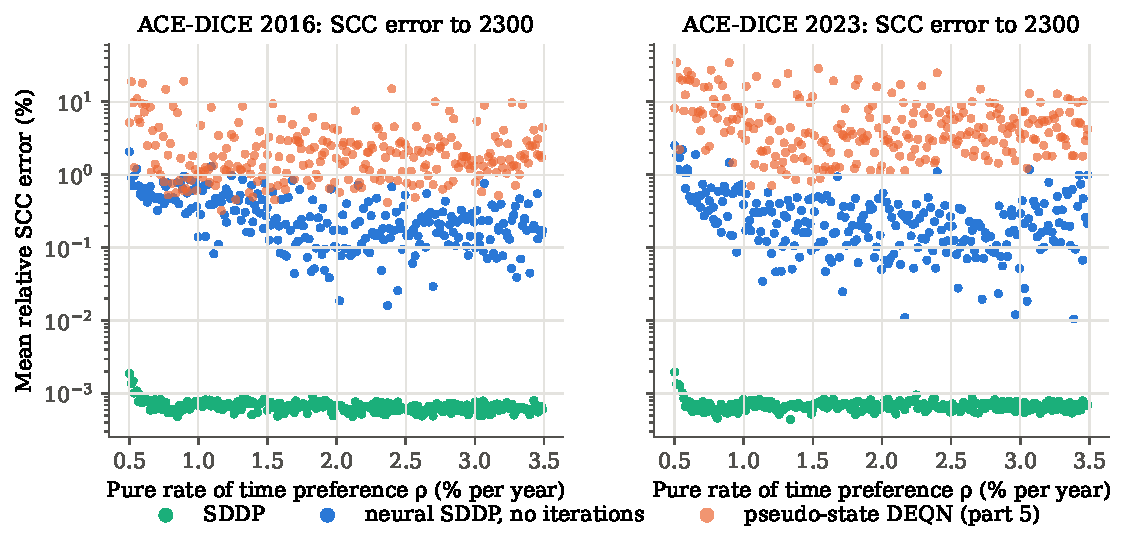
\includegraphics[width=\textwidth]{accuracy.pdf}
\caption{Mean relative SCC error over the evaluation window on the 256 test instances, against the time preference, for SDDP, neural SDDP without iterations, and the pseudo-state deep equilibrium net. Log scale.}
\label{fig:accuracy}
\end{figure}

\begin{figure}[t]
\centering
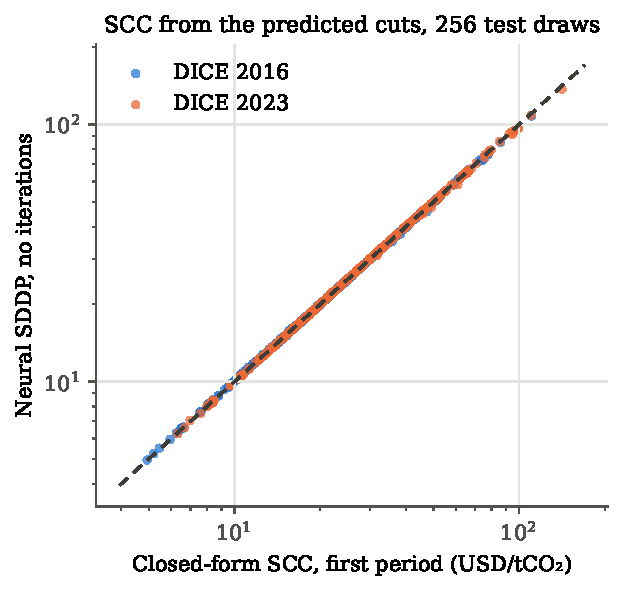
\includegraphics[width=0.55\textwidth]{parity.pdf}
\caption{SCC in the first period from the predicted cuts, against the closed form, on the 256 test instances of both calibrations.}
\label{fig:parity}
\end{figure}

\begin{figure}[t]
\centering
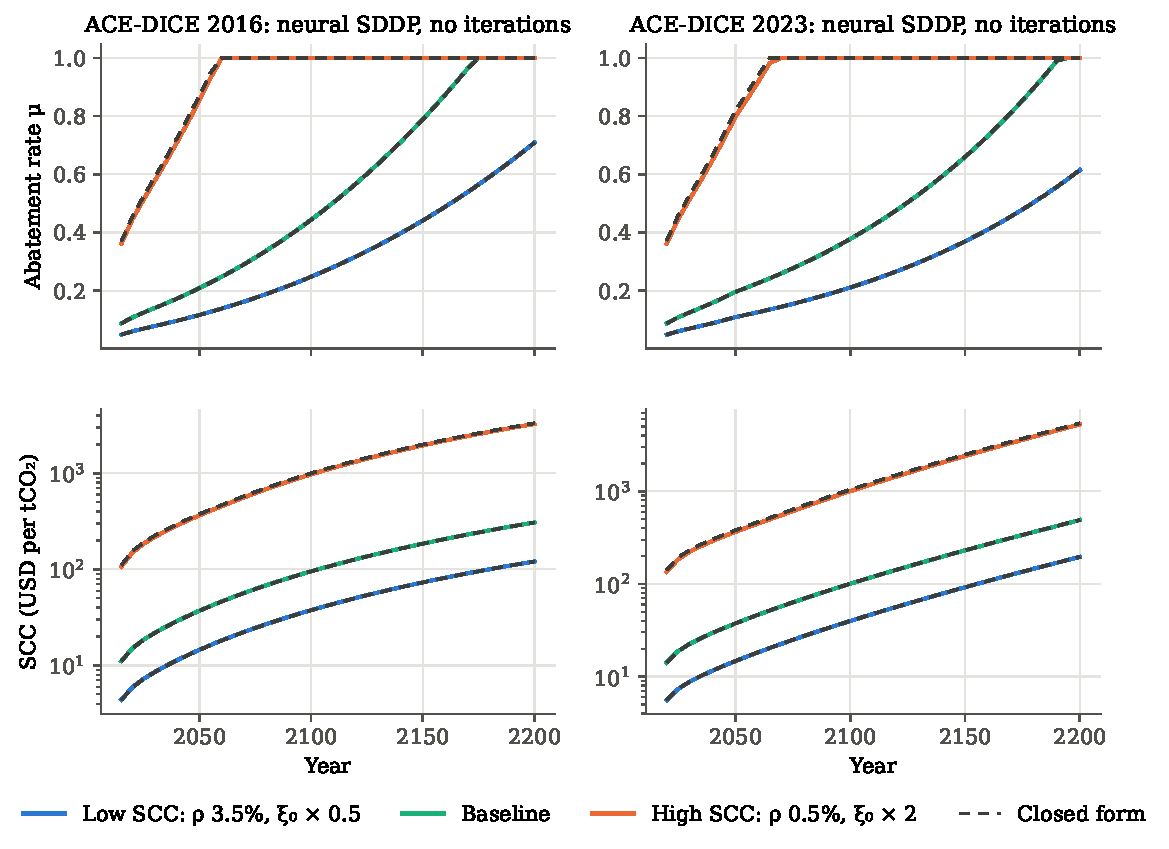
\includegraphics[width=\textwidth]{paths.pdf}
\caption{Abatement rate and SCC from neural SDDP without iterations (solid) and the closed form (dashed), for three instances: low SCC ($\rho = 3.5\%$, half the baseline damages), baseline, and high SCC ($\rho = 0.5\%$, twice the baseline damages).}
\label{fig:paths}
\end{figure}

\subsection{Comparison with a pseudo-state deep equilibrium net}

On the same test instances, the pseudo-state deep equilibrium net has a median SCC error of 1.8\% for DICE 2016 and 4.0\% for DICE 2023, and at most 19\% and 35\%. Neural SDDP without iterations is 8 to 19 times more accurate in the median and 9 to 14 times in the worst case, and its abatement errors are 10 to 35 times smaller (Table~\ref{tab:accuracy}, Figure~\ref{fig:accuracy}). Its training is also cheaper: 90 seconds of SDDP for the training data and 11 minutes for the network, against 53 minutes for the deep equilibrium net (38 minutes for DICE 2023), all on four CPU cores. Section~\ref{sec:discussion} discusses why this comparison favours neural SDDP.

\subsection{Warm starts}

\begin{figure}[t]
\centering
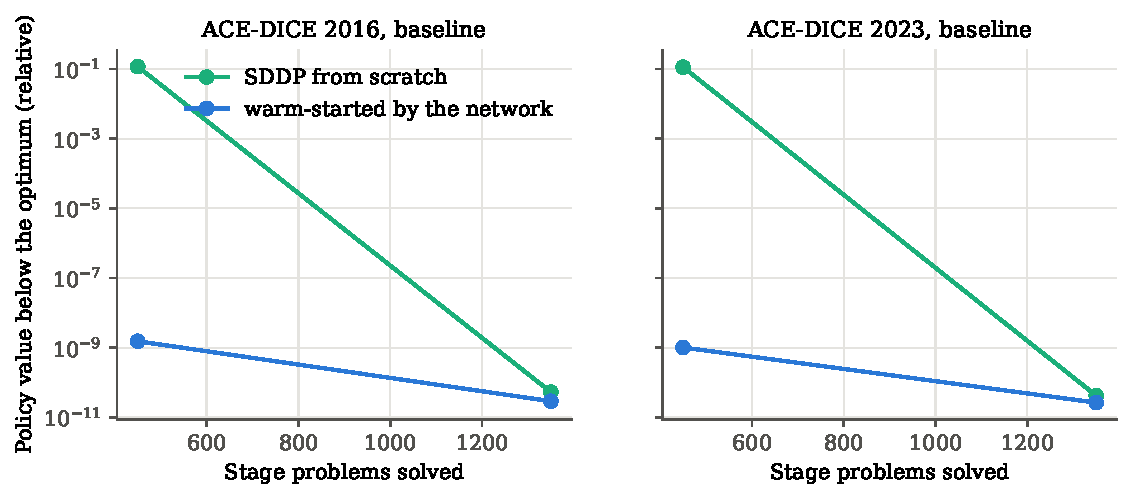
\includegraphics[width=\textwidth]{convergence.pdf}
\caption{Relative shortfall of the forward-pass value from the optimum at baseline parameters, against the number of stage problems solved, for SDDP from scratch and warm-started with the predicted cuts. Log scale; each marker is one iteration.}
\label{fig:convergence}
\end{figure}

With the predicted cuts, the first forward pass is already nearly optimal: its value is within $1.5 \times 10^{-9}$ (DICE 2016) and $1.0 \times 10^{-9}$ (DICE 2023) of the optimum, against 11.7\% below it for SDDP from scratch, whose first forward pass is driven only by the provisional bound (Figure~\ref{fig:convergence}). But the predicted cuts are not guaranteed to lie above the value function, so they cannot certify convergence; a backward pass is needed either way. SDDP from scratch needs exactly one (Corollary~\ref{cor:two}), and both variants finish after two iterations, with the same 1{,}350 stage problems and the same accuracy (Table~\ref{tab:cost}).

\subsection{Productivity shocks}

With i.i.d.\ shocks to log productivity with a standard deviation of 3\%, SDDP runs six iterations of 2{,}700 stage problems each (16{,}200 in total, 31 seconds): forward passes along sampled shocks and backward passes over five Gauss--Hermite nodes. The cut slopes match the closed form to $10^{-14}$, and along a sampled path, on which log capital deviates from the deterministic optimum by up to 0.07, the decisions match the deterministic optimal policy to within $3 \times 10^{-5}$ for the consumption rate and $10^{-4}$ for the abatement rate. As ACE predicts, the shocks shift the value function but not its slopes, and with it, not the policy.

\section{Discussion}
\label{sec:discussion}

\paragraph{Three routes to the same shadow price.} In ACE, the SCC is a ratio of costates, and the three families of methods studied in this series reach the costates in different ways. Deep equilibrium nets learn them as outputs that satisfy the residuals of the equilibrium conditions. Actor-critic methods obtain them as the gradient of a learned value function. SDDP computes them from the duals of convex stage problems, and Proposition~\ref{prop:gradient} shows that this is the same costate recursion that the equilibrium conditions encode, evaluated exactly at a visited state instead of enforced approximately over a distribution of states. Seen this way, SDDP is a form of approximate dynamic programming in which the value function is represented by cuts and improved with exact dual information; its accuracy in ACE comes from the fact that this representation contains the true value function.

\paragraph{Why ACE is easy for SDDP.} SDDP suits ACE unusually well: two decisions per period, convex stage problems, and an affine value function that a single cut represents exactly. Corollary~\ref{cor:two} turns this into convergence after one backward pass. This is a strength of the benchmark, since every result can be verified, but it also means that ACE does not test what makes SDDP hard in general: value functions that need many cuts, high-dimensional decisions, and many scenarios per stage. The two-iteration convergence and the absent warm-start gains should be read in that light. They say that neural SDDP cannot improve on an exact method that is already fast, not that warm starts are useless.

\paragraph{What the comparison with the deep equilibrium net shows.} Neural SDDP without iterations is about an order of magnitude more accurate than the pseudo-state deep equilibrium net on the same instances, at a quarter to a third of the training time. The comparison favours neural SDDP in two ways. First, its network is trained by supervised learning on exact solutions, which exist only because SDDP can solve every training instance; the deep equilibrium net learns from the equilibrium conditions alone and needs no solver. Second, the cut network has an easy target: a smooth map from three parameters and the period to six slopes and an intercept, the same at every state. The deep equilibrium net must represent policies and costates as functions of the full state, and its accuracy depends on where its simulated states fall. The fairer reading is that, when a convex solver can generate training data, learning the solution of the dual problem is much easier than learning the solution of the equilibrium conditions. Both approaches remain cheap to evaluate: the first-period SCC of a new instance needs only the predicted cut for period one and a single stage problem, so uncertainty quantification over many parameter draws is as feasible with neural SDDP as with the pseudo-state network.

\paragraph{Limits.} The results rest on three assumptions. The first is convexity. The stage problems are convex only because business-as-usual emissions follow an exogenous path; if they are tied to capital, as in DICE, emissions become a product of the abatement rate and a convex function of capital, the value function need not be concave in the state, and cuts are no longer valid upper bounds. Tipping points with thresholds or regime switches \parencite{LemoineTraeger2014,CaiLontzek2019} break convexity in the same way. SDDP can still be run as a heuristic in such models, but without its bounds, and neural SDDP inherits that. The second is stagewise independence: SDDP handles i.i.d.\ shocks directly, but persistent shocks or learning about uncertain parameters require adding states, which in turn makes the value functions curved. The third is the finite horizon: as Remark~\ref{rem:truncation} shows, carbon's shadow price converges only at the rate of discounting, so low discount rates require horizons of thousands of years, or a terminal value function. Finally, the cut network is trained with one seed per calibration, and I have not explored how many training instances are needed.

\paragraph{Where neural SDDP should pay off.} The case for neural SDDP is strongest exactly where ACE stops being a good benchmark: models whose value functions are curved enough to need many cuts, so that SDDP needs many iterations and good initial cuts save most of them. A natural next step is a convex extension of ACE that keeps a closed form for part of the problem, for example stochastic damages with a convex hazard, followed by models without closed forms, for which the methods validated here would themselves become the benchmark.

\section{Conclusion}
\label{sec:conclusion}

With business-as-usual emissions taken as given, the Analytic Climate Economy decomposes into convex stage problems whose cut slopes are its costates. SDDP solves it exactly in two iterations, recovering the closed-form social cost of carbon to within 0.002\% across a wide range of time preferences, damages and carbon-cycle parameters, and with productivity shocks it recovers the same costates and policy. Neural SDDP, trained on 128 SDDP solutions, predicts the cuts of new instances accurately enough that a single forward pass gives the SCC within 0.2\% in the median, an order of magnitude more accurately than a pseudo-state deep equilibrium net. Its warm starts, the main source of speed-ups in the operations-research literature, do not help here, because the affine value function of ACE leaves SDDP nothing to gain. The lesson for climate economics is twofold: where a model is convex, cutting-plane methods offer exact, certifiable solutions and an easy target for learning; and the interesting tests for neural SDDP lie in the models, with curved value functions and uncertainty, that ACE was designed to avoid.


\section*{Code and Data Availability}
All code, data and results are available at \url{https://github.com/hermanvest/DNN-for-ACE} in the directory \texttt{6\_neural\_sddp/}.

\printbibliography

\end{document}
